%% ENGR114 Lab 8 External Hardware

%preamble.tex


%% installed packages_rev2.tplx %%

\usepackage{fancyhdr}
\usepackage{lastpage}
\usepackage{framed,color}
\definecolor{shadecolor}{rgb}{.8,.8,.8}
\usepackage{titlesec}
\usepackage{listings}
% no indent on any paragraphs, vertical spacing between paragraphs is set to 1em
\usepackage[]{parskip}  % add [skip=1em] if the compiler will allow.

% for MATLAB syntax highlighting
\usepackage{listings}             % Include the listings-package
\definecolor{mygray}{rgb}{0.8,0.8,0.8} % color values Red, Green, Blue
\definecolor{mygreen}{RGB}{28,172,0}
\definecolor{mylilas}{RGB}{170,55,241}
    
    \usepackage[T1]{fontenc}
    % Nicer default font (+ math font) than Computer Modern for most use cases
    \usepackage{mathpazo}

    % Basic figure setup, for now with no caption control since it's done
    % automatically by Pandoc (which extracts ![](path) syntax from Markdown).
    \usepackage{graphicx}
    % We will generate all images so they have a width \maxwidth. This means
    % that they will get their normal width if they fit onto the page, but
    % are scaled down if they would overflow the margins.
    \makeatletter
    \def\maxwidth{\ifdim\Gin@nat@width>\linewidth\linewidth
    \else\Gin@nat@width\fi}
    \makeatother
    \let\Oldincludegraphics\includegraphics
    % Set max figure width to be 80% of text width, for now hardcoded.
   % \renewcommand{\includegraphics}[1]{\Oldincludegraphics[width=.8\maxwidth]{#1}}
    % Ensure that by default, figures have no caption (until we provide a
    % proper Figure object with a Caption API and a way to capture that
    % in the conversion process - todo).
    \usepackage{caption}
    \DeclareCaptionLabelFormat{nolabel}{}
    \captionsetup{labelformat=nolabel}

    \usepackage{adjustbox} % Used to constrain images to a maximum size 
    \usepackage{xcolor} % Allow colors to be defined
    \usepackage{enumerate} % Needed for markdown enumerations to work
    \usepackage{geometry} % Used to adjust the document margins
    \usepackage{amsmath} % Equations
    \usepackage{amssymb} % Equations
    \usepackage{textcomp} % defines textquotesingle
    % Hack from http://tex.stackexchange.com/a/47451/13684:
    \AtBeginDocument{%
        \def\PYZsq{\textquotesingle}% Upright quotes in Pygmentized code
    }
    \usepackage{upquote} % Upright quotes for verbatim code
    \usepackage{eurosym} % defines \euro
    \usepackage[mathletters]{ucs} % Extended unicode (utf-8) support
    \usepackage[utf8x]{inputenc} % Allow utf-8 characters in the tex document
    \usepackage{fancyvrb} % verbatim replacement that allows latex
    \usepackage{grffile} % extends the file name processing of package graphics 
                         % to support a larger range 
    % The hyperref package gives us a pdf with properly built
    % internal navigation ('pdf bookmarks' for the table of contents,
    % internal cross-reference links, web links for URLs, etc.)
    \usepackage{hyperref}
    \usepackage{longtable} % longtable support required by pandoc >1.10
    \usepackage{booktabs}  % table support for pandoc > 1.12.2
    \usepackage[inline]{enumitem} % IRkernel/repr support (it uses the enumerate* environment)
    \usepackage[normalem]{ulem} % ulem is needed to support strikethroughs (\sout)
                                % normalem makes italics be italics, not underlines
    


    
    %% lab_title.tplx %% 
 
\newcommand{\labtitle}{Lab06 Image Filtering} 
    %% header_and_footer.tplx %%

% Header and Footer
\lhead{\textbf{\labtitle}}
\rhead{ENGR114 Engineering Programming}
\lfoot{Portland Community College, \the\year}
\cfoot{}
\rfoot{\thepage~of~\pageref{LastPage}}  % must compile twice for LastPage

%lines below header and above footer
\renewcommand{\headrulewidth}{0.4pt}
\renewcommand{\footrulewidth}{0.4pt}

% Tabs
\newcommand{\itab}[1]{\hspace{0em}\rlap{#1}}
\newcommand{\tab}[1]{\hspace{.4\textwidth}\rlap{#1}}
\newcommand{\tabA}[1]{\hspace{.2\textwidth}\rlap{#1}}
    %% title_sec_formatting.tplx %%

\titleformat{\section}[block]{\LARGE\bfseries\filcenter}{}{1em}{}

\titleformat{\subsection}[hang]{\Large\bfseries}{}{1em}{}
\titlespacing{\subsection}{-1.4em}{1.5em}{1em}

\titleformat{\subsubsection}[hang]{\large\bfseries}{}{1em}{}
\titlespacing{\subsubsection}{-1.1em}{1.5em}{0.8em}
    
        \title{Problem Solving 101 with Python}
        \author{Peter D. Kazarinoff, PhD}
        \date{}
    
    
    
    % Colors for the hyperref package
    \definecolor{urlcolor}{rgb}{0,.145,.698}
    \definecolor{linkcolor}{rgb}{.71,0.21,0.01}
    \definecolor{citecolor}{rgb}{.12,.54,.11}

    % ANSI colors
    \definecolor{ansi-black}{HTML}{3E424D}
    \definecolor{ansi-black-intense}{HTML}{282C36}
    \definecolor{ansi-red}{HTML}{E75C58}
    \definecolor{ansi-red-intense}{HTML}{B22B31}
    \definecolor{ansi-green}{HTML}{00A250}
    \definecolor{ansi-green-intense}{HTML}{007427}
    \definecolor{ansi-yellow}{HTML}{DDB62B}
    \definecolor{ansi-yellow-intense}{HTML}{B27D12}
    \definecolor{ansi-blue}{HTML}{208FFB}
    \definecolor{ansi-blue-intense}{HTML}{0065CA}
    \definecolor{ansi-magenta}{HTML}{D160C4}
    \definecolor{ansi-magenta-intense}{HTML}{A03196}
    \definecolor{ansi-cyan}{HTML}{60C6C8}
    \definecolor{ansi-cyan-intense}{HTML}{258F8F}
    \definecolor{ansi-white}{HTML}{C5C1B4}
    \definecolor{ansi-white-intense}{HTML}{A1A6B2}

    % commands and environments needed by pandoc snippets
    % extracted from the output of `pandoc -s`
    \providecommand{\tightlist}{%
      \setlength{\itemsep}{0pt}\setlength{\parskip}{0pt}}
    \DefineVerbatimEnvironment{Highlighting}{Verbatim}{commandchars=\\\{\}}
    % Add ',fontsize=\small' for more characters per line
    \newenvironment{Shaded}{}{}
    \newcommand{\KeywordTok}[1]{\textcolor[rgb]{0.00,0.44,0.13}{\textbf{{#1}}}}
    \newcommand{\DataTypeTok}[1]{\textcolor[rgb]{0.56,0.13,0.00}{{#1}}}
    \newcommand{\DecValTok}[1]{\textcolor[rgb]{0.25,0.63,0.44}{{#1}}}
    \newcommand{\BaseNTok}[1]{\textcolor[rgb]{0.25,0.63,0.44}{{#1}}}
    \newcommand{\FloatTok}[1]{\textcolor[rgb]{0.25,0.63,0.44}{{#1}}}
    \newcommand{\CharTok}[1]{\textcolor[rgb]{0.25,0.44,0.63}{{#1}}}
    \newcommand{\StringTok}[1]{\textcolor[rgb]{0.25,0.44,0.63}{{#1}}}
    \newcommand{\CommentTok}[1]{\textcolor[rgb]{0.38,0.63,0.69}{\textit{{#1}}}}
    \newcommand{\OtherTok}[1]{\textcolor[rgb]{0.00,0.44,0.13}{{#1}}}
    \newcommand{\AlertTok}[1]{\textcolor[rgb]{1.00,0.00,0.00}{\textbf{{#1}}}}
    \newcommand{\FunctionTok}[1]{\textcolor[rgb]{0.02,0.16,0.49}{{#1}}}
    \newcommand{\RegionMarkerTok}[1]{{#1}}
    \newcommand{\ErrorTok}[1]{\textcolor[rgb]{1.00,0.00,0.00}{\textbf{{#1}}}}
    \newcommand{\NormalTok}[1]{{#1}}
    
    % Additional commands for more recent versions of Pandoc
    \newcommand{\ConstantTok}[1]{\textcolor[rgb]{0.53,0.00,0.00}{{#1}}}
    \newcommand{\SpecialCharTok}[1]{\textcolor[rgb]{0.25,0.44,0.63}{{#1}}}
    \newcommand{\VerbatimStringTok}[1]{\textcolor[rgb]{0.25,0.44,0.63}{{#1}}}
    \newcommand{\SpecialStringTok}[1]{\textcolor[rgb]{0.73,0.40,0.53}{{#1}}}
    \newcommand{\ImportTok}[1]{{#1}}
    \newcommand{\DocumentationTok}[1]{\textcolor[rgb]{0.73,0.13,0.13}{\textit{{#1}}}}
    \newcommand{\AnnotationTok}[1]{\textcolor[rgb]{0.38,0.63,0.69}{\textbf{\textit{{#1}}}}}
    \newcommand{\CommentVarTok}[1]{\textcolor[rgb]{0.38,0.63,0.69}{\textbf{\textit{{#1}}}}}
    \newcommand{\VariableTok}[1]{\textcolor[rgb]{0.10,0.09,0.49}{{#1}}}
    \newcommand{\ControlFlowTok}[1]{\textcolor[rgb]{0.00,0.44,0.13}{\textbf{{#1}}}}
    \newcommand{\OperatorTok}[1]{\textcolor[rgb]{0.40,0.40,0.40}{{#1}}}
    \newcommand{\BuiltInTok}[1]{{#1}}
    \newcommand{\ExtensionTok}[1]{{#1}}
    \newcommand{\PreprocessorTok}[1]{\textcolor[rgb]{0.74,0.48,0.00}{{#1}}}
    \newcommand{\AttributeTok}[1]{\textcolor[rgb]{0.49,0.56,0.16}{{#1}}}
    \newcommand{\InformationTok}[1]{\textcolor[rgb]{0.38,0.63,0.69}{\textbf{\textit{{#1}}}}}
    \newcommand{\WarningTok}[1]{\textcolor[rgb]{0.38,0.63,0.69}{\textbf{\textit{{#1}}}}}
    
    
    % Define a nice break command that doesn't care if a line doesn't already
    % exist.
    \def\br{\hspace*{\fill} \\* }
    % Math Jax compatability definitions
    \def\gt{>}
    \def\lt{<}
    % Document parameters
    
        \title{Problem Solving 101 with Python}
        \author{Peter D. Kazarinoff, PhD}
        \date{}
    
    
    
    

    % Pygments definitions
    
\makeatletter
\def\PY@reset{\let\PY@it=\relax \let\PY@bf=\relax%
    \let\PY@ul=\relax \let\PY@tc=\relax%
    \let\PY@bc=\relax \let\PY@ff=\relax}
\def\PY@tok#1{\csname PY@tok@#1\endcsname}
\def\PY@toks#1+{\ifx\relax#1\empty\else%
    \PY@tok{#1}\expandafter\PY@toks\fi}
\def\PY@do#1{\PY@bc{\PY@tc{\PY@ul{%
    \PY@it{\PY@bf{\PY@ff{#1}}}}}}}
\def\PY#1#2{\PY@reset\PY@toks#1+\relax+\PY@do{#2}}

\expandafter\def\csname PY@tok@w\endcsname{\def\PY@tc##1{\textcolor[rgb]{0.73,0.73,0.73}{##1}}}
\expandafter\def\csname PY@tok@c\endcsname{\let\PY@it=\textit\def\PY@tc##1{\textcolor[rgb]{0.25,0.50,0.50}{##1}}}
\expandafter\def\csname PY@tok@cp\endcsname{\def\PY@tc##1{\textcolor[rgb]{0.74,0.48,0.00}{##1}}}
\expandafter\def\csname PY@tok@k\endcsname{\let\PY@bf=\textbf\def\PY@tc##1{\textcolor[rgb]{0.00,0.50,0.00}{##1}}}
\expandafter\def\csname PY@tok@kp\endcsname{\def\PY@tc##1{\textcolor[rgb]{0.00,0.50,0.00}{##1}}}
\expandafter\def\csname PY@tok@kt\endcsname{\def\PY@tc##1{\textcolor[rgb]{0.69,0.00,0.25}{##1}}}
\expandafter\def\csname PY@tok@o\endcsname{\def\PY@tc##1{\textcolor[rgb]{0.40,0.40,0.40}{##1}}}
\expandafter\def\csname PY@tok@ow\endcsname{\let\PY@bf=\textbf\def\PY@tc##1{\textcolor[rgb]{0.67,0.13,1.00}{##1}}}
\expandafter\def\csname PY@tok@nb\endcsname{\def\PY@tc##1{\textcolor[rgb]{0.00,0.50,0.00}{##1}}}
\expandafter\def\csname PY@tok@nf\endcsname{\def\PY@tc##1{\textcolor[rgb]{0.00,0.00,1.00}{##1}}}
\expandafter\def\csname PY@tok@nc\endcsname{\let\PY@bf=\textbf\def\PY@tc##1{\textcolor[rgb]{0.00,0.00,1.00}{##1}}}
\expandafter\def\csname PY@tok@nn\endcsname{\let\PY@bf=\textbf\def\PY@tc##1{\textcolor[rgb]{0.00,0.00,1.00}{##1}}}
\expandafter\def\csname PY@tok@ne\endcsname{\let\PY@bf=\textbf\def\PY@tc##1{\textcolor[rgb]{0.82,0.25,0.23}{##1}}}
\expandafter\def\csname PY@tok@nv\endcsname{\def\PY@tc##1{\textcolor[rgb]{0.10,0.09,0.49}{##1}}}
\expandafter\def\csname PY@tok@no\endcsname{\def\PY@tc##1{\textcolor[rgb]{0.53,0.00,0.00}{##1}}}
\expandafter\def\csname PY@tok@nl\endcsname{\def\PY@tc##1{\textcolor[rgb]{0.63,0.63,0.00}{##1}}}
\expandafter\def\csname PY@tok@ni\endcsname{\let\PY@bf=\textbf\def\PY@tc##1{\textcolor[rgb]{0.60,0.60,0.60}{##1}}}
\expandafter\def\csname PY@tok@na\endcsname{\def\PY@tc##1{\textcolor[rgb]{0.49,0.56,0.16}{##1}}}
\expandafter\def\csname PY@tok@nt\endcsname{\let\PY@bf=\textbf\def\PY@tc##1{\textcolor[rgb]{0.00,0.50,0.00}{##1}}}
\expandafter\def\csname PY@tok@nd\endcsname{\def\PY@tc##1{\textcolor[rgb]{0.67,0.13,1.00}{##1}}}
\expandafter\def\csname PY@tok@s\endcsname{\def\PY@tc##1{\textcolor[rgb]{0.73,0.13,0.13}{##1}}}
\expandafter\def\csname PY@tok@sd\endcsname{\let\PY@it=\textit\def\PY@tc##1{\textcolor[rgb]{0.73,0.13,0.13}{##1}}}
\expandafter\def\csname PY@tok@si\endcsname{\let\PY@bf=\textbf\def\PY@tc##1{\textcolor[rgb]{0.73,0.40,0.53}{##1}}}
\expandafter\def\csname PY@tok@se\endcsname{\let\PY@bf=\textbf\def\PY@tc##1{\textcolor[rgb]{0.73,0.40,0.13}{##1}}}
\expandafter\def\csname PY@tok@sr\endcsname{\def\PY@tc##1{\textcolor[rgb]{0.73,0.40,0.53}{##1}}}
\expandafter\def\csname PY@tok@ss\endcsname{\def\PY@tc##1{\textcolor[rgb]{0.10,0.09,0.49}{##1}}}
\expandafter\def\csname PY@tok@sx\endcsname{\def\PY@tc##1{\textcolor[rgb]{0.00,0.50,0.00}{##1}}}
\expandafter\def\csname PY@tok@m\endcsname{\def\PY@tc##1{\textcolor[rgb]{0.40,0.40,0.40}{##1}}}
\expandafter\def\csname PY@tok@gh\endcsname{\let\PY@bf=\textbf\def\PY@tc##1{\textcolor[rgb]{0.00,0.00,0.50}{##1}}}
\expandafter\def\csname PY@tok@gu\endcsname{\let\PY@bf=\textbf\def\PY@tc##1{\textcolor[rgb]{0.50,0.00,0.50}{##1}}}
\expandafter\def\csname PY@tok@gd\endcsname{\def\PY@tc##1{\textcolor[rgb]{0.63,0.00,0.00}{##1}}}
\expandafter\def\csname PY@tok@gi\endcsname{\def\PY@tc##1{\textcolor[rgb]{0.00,0.63,0.00}{##1}}}
\expandafter\def\csname PY@tok@gr\endcsname{\def\PY@tc##1{\textcolor[rgb]{1.00,0.00,0.00}{##1}}}
\expandafter\def\csname PY@tok@ge\endcsname{\let\PY@it=\textit}
\expandafter\def\csname PY@tok@gs\endcsname{\let\PY@bf=\textbf}
\expandafter\def\csname PY@tok@gp\endcsname{\let\PY@bf=\textbf\def\PY@tc##1{\textcolor[rgb]{0.00,0.00,0.50}{##1}}}
\expandafter\def\csname PY@tok@go\endcsname{\def\PY@tc##1{\textcolor[rgb]{0.53,0.53,0.53}{##1}}}
\expandafter\def\csname PY@tok@gt\endcsname{\def\PY@tc##1{\textcolor[rgb]{0.00,0.27,0.87}{##1}}}
\expandafter\def\csname PY@tok@err\endcsname{\def\PY@bc##1{\setlength{\fboxsep}{0pt}\fcolorbox[rgb]{1.00,0.00,0.00}{1,1,1}{\strut ##1}}}
\expandafter\def\csname PY@tok@kc\endcsname{\let\PY@bf=\textbf\def\PY@tc##1{\textcolor[rgb]{0.00,0.50,0.00}{##1}}}
\expandafter\def\csname PY@tok@kd\endcsname{\let\PY@bf=\textbf\def\PY@tc##1{\textcolor[rgb]{0.00,0.50,0.00}{##1}}}
\expandafter\def\csname PY@tok@kn\endcsname{\let\PY@bf=\textbf\def\PY@tc##1{\textcolor[rgb]{0.00,0.50,0.00}{##1}}}
\expandafter\def\csname PY@tok@kr\endcsname{\let\PY@bf=\textbf\def\PY@tc##1{\textcolor[rgb]{0.00,0.50,0.00}{##1}}}
\expandafter\def\csname PY@tok@bp\endcsname{\def\PY@tc##1{\textcolor[rgb]{0.00,0.50,0.00}{##1}}}
\expandafter\def\csname PY@tok@fm\endcsname{\def\PY@tc##1{\textcolor[rgb]{0.00,0.00,1.00}{##1}}}
\expandafter\def\csname PY@tok@vc\endcsname{\def\PY@tc##1{\textcolor[rgb]{0.10,0.09,0.49}{##1}}}
\expandafter\def\csname PY@tok@vg\endcsname{\def\PY@tc##1{\textcolor[rgb]{0.10,0.09,0.49}{##1}}}
\expandafter\def\csname PY@tok@vi\endcsname{\def\PY@tc##1{\textcolor[rgb]{0.10,0.09,0.49}{##1}}}
\expandafter\def\csname PY@tok@vm\endcsname{\def\PY@tc##1{\textcolor[rgb]{0.10,0.09,0.49}{##1}}}
\expandafter\def\csname PY@tok@sa\endcsname{\def\PY@tc##1{\textcolor[rgb]{0.73,0.13,0.13}{##1}}}
\expandafter\def\csname PY@tok@sb\endcsname{\def\PY@tc##1{\textcolor[rgb]{0.73,0.13,0.13}{##1}}}
\expandafter\def\csname PY@tok@sc\endcsname{\def\PY@tc##1{\textcolor[rgb]{0.73,0.13,0.13}{##1}}}
\expandafter\def\csname PY@tok@dl\endcsname{\def\PY@tc##1{\textcolor[rgb]{0.73,0.13,0.13}{##1}}}
\expandafter\def\csname PY@tok@s2\endcsname{\def\PY@tc##1{\textcolor[rgb]{0.73,0.13,0.13}{##1}}}
\expandafter\def\csname PY@tok@sh\endcsname{\def\PY@tc##1{\textcolor[rgb]{0.73,0.13,0.13}{##1}}}
\expandafter\def\csname PY@tok@s1\endcsname{\def\PY@tc##1{\textcolor[rgb]{0.73,0.13,0.13}{##1}}}
\expandafter\def\csname PY@tok@mb\endcsname{\def\PY@tc##1{\textcolor[rgb]{0.40,0.40,0.40}{##1}}}
\expandafter\def\csname PY@tok@mf\endcsname{\def\PY@tc##1{\textcolor[rgb]{0.40,0.40,0.40}{##1}}}
\expandafter\def\csname PY@tok@mh\endcsname{\def\PY@tc##1{\textcolor[rgb]{0.40,0.40,0.40}{##1}}}
\expandafter\def\csname PY@tok@mi\endcsname{\def\PY@tc##1{\textcolor[rgb]{0.40,0.40,0.40}{##1}}}
\expandafter\def\csname PY@tok@il\endcsname{\def\PY@tc##1{\textcolor[rgb]{0.40,0.40,0.40}{##1}}}
\expandafter\def\csname PY@tok@mo\endcsname{\def\PY@tc##1{\textcolor[rgb]{0.40,0.40,0.40}{##1}}}
\expandafter\def\csname PY@tok@ch\endcsname{\let\PY@it=\textit\def\PY@tc##1{\textcolor[rgb]{0.25,0.50,0.50}{##1}}}
\expandafter\def\csname PY@tok@cm\endcsname{\let\PY@it=\textit\def\PY@tc##1{\textcolor[rgb]{0.25,0.50,0.50}{##1}}}
\expandafter\def\csname PY@tok@cpf\endcsname{\let\PY@it=\textit\def\PY@tc##1{\textcolor[rgb]{0.25,0.50,0.50}{##1}}}
\expandafter\def\csname PY@tok@c1\endcsname{\let\PY@it=\textit\def\PY@tc##1{\textcolor[rgb]{0.25,0.50,0.50}{##1}}}
\expandafter\def\csname PY@tok@cs\endcsname{\let\PY@it=\textit\def\PY@tc##1{\textcolor[rgb]{0.25,0.50,0.50}{##1}}}

\def\PYZbs{\char`\\}
\def\PYZus{\char`\_}
\def\PYZob{\char`\{}
\def\PYZcb{\char`\}}
\def\PYZca{\char`\^}
\def\PYZam{\char`\&}
\def\PYZlt{\char`\<}
\def\PYZgt{\char`\>}
\def\PYZsh{\char`\#}
\def\PYZpc{\char`\%}
\def\PYZdl{\char`\$}
\def\PYZhy{\char`\-}
\def\PYZsq{\char`\'}
\def\PYZdq{\char`\"}
\def\PYZti{\char`\~}
% for compatibility with earlier versions
\def\PYZat{@}
\def\PYZlb{[}
\def\PYZrb{]}
\makeatother


    % Exact colors from NB
    \definecolor{incolor}{rgb}{0.0, 0.0, 0.5}
    \definecolor{outcolor}{rgb}{0.545, 0.0, 0.0}




    
    % Prevent overflowing lines due to hard-to-break entities
    \sloppy 
    % Setup hyperref package
    \hypersetup{
      breaklinks=true,  % so long urls are correctly broken across lines
      colorlinks=true,
      urlcolor=urlcolor,
      linkcolor=linkcolor,
      citecolor=citecolor,
      }
    % Slightly bigger margins than the latex defaults
    
    %% margins.tplx %%

% margins
\textwidth=7in
\textheight=9.0in
\topmargin=-0.5in
\headheight=15pt
\headsep=.5in
\hoffset = -0.5in

\pagestyle{fancy}

    
\begin{document}

\hypertarget{lab-08---external-hardware}{%
\section{Lab 08 - External Hardware}\label{lab-08---external-hardware}}

In this lab, you will use Python to communicate to a piece of external
hardware.

\hypertarget{prelab}{%
\subsection{Prelab}\label{prelab}}

Before starting the lab, familiarize yourself with what an Arduino is
and what an Arduino can be used for. You will find numerous projects if
you Google ``Arduino project''. Download the Arduino IDE using the
following link:

\begin{quote}
\href{https://www.arduino.cc/en/Main/Software}{https://www.arduino.cc/en/Main/Software}
\end{quote}

Be sure to select: \textbf{{[}Windows ZIP file for non admin install{]}}
as new software can not be installed on lab computers without
administrator privileges.

\begin{figure}[h!]
\centering

\includegraphics{images/arduino_download_page.png}
\caption{Arduino IDE Download Page}
\end{figure}

Investigate the Arudino IDE (launch by double clicking
\textbf{Arduino.exe}). See what is available in the {[}File{]}
--\textgreater{} {[}Examples{]} menu. Before lab, also familiarize
yourself with the concept of serial communication. In this lab, Python
will communicate with an Arduino over a serial connection. Serial
communication is one of the older computer hardware communication
specifications. Serial communication is a precursor to USB (universal
\emph{serial} bus) communication used by keyboards, mice, printers,
thumb drives etc.

The first part of this lab will follow a tutorial from the Sparkfun
Inventor's Kit:

\begin{quote}
\href{https://www.sparkfun.com/products/retired/12060}{https://www.sparkfun.com/products/retired/12060}
\end{quote}

Click on the \textbf{{[}Documents{]}} link on the product page to review
the guide.

\newpage

    \hypertarget{lab}{%
\subsection{Lab}\label{lab}}

For this group lab assignment, your group will use Python to interact
with an Arduino to dynamically turn on and off an LED, and then your
group will use Python to collect and plot the sensor data. Your group
will construct two Python scripts and use two Arduino scripts to
complete these tasks. At the end of the lab, you will be able to use
Python to interact with external hardware.

    An outline of the steps to complete the lab is below:

\hypertarget{part-1-turn-an-led-on-and-off-with-python-and-an-arduino}{%
\subsubsection{Part 1: Turn an LED on and off with Python and an
Arduino}\label{part-1-turn-an-led-on-and-off-with-python-and-an-arduino}}

\begin{enumerate}
\def\labelenumi{(\alph{enumi})}
\item
  Download the Arduino IDE
\item
  Wire an LED and resistor to the Arduino
\item
  Upload the Arduino example sketch \textbf{\emph{blink.ino}} onto the
  Arduino. Confirm your Arduino and LED blinks.
\item
  Load the Arduino example sketch \textbf{\emph{PhysicalPixel.ino}} onto
  the Arduino
\item
  Use the serial monitor to turn the Arduino LED on and off
\item
  Build a Python script to turn the Arduino LED on and off
\end{enumerate}

    \hypertarget{part-2-measure-sensor-output-with-python-and-an-arduino}{%
\subsubsection{Part 2: Measure sensor output with Python and an
Arduino}\label{part-2-measure-sensor-output-with-python-and-an-arduino}}

\begin{enumerate}
\def\labelenumi{(\alph{enumi})}
\item
  Wire a little blue potentiometer dial to the Arduino
\item
  Copy and load the \textbf{\emph{potentiometer.ino}} sketch onto the
  Arduino
\item
  Twist the little blue potentiometer to turn the LED connected to the
  Arduino on and off
\item
  Use the Arduino Serial Monitor and Arduino Serial Plotter to see the
  potentiometer reading
\item
  Build a Python script and to record the potentiometer level and draw a
  plot
\end{enumerate}

    You will complete this lab in groups. Below are details for each of the
steps outlined above.

\newpage

\hypertarget{part-1.-turn-an-led-on-and-off-with-python-and-an-arduino}{%
\subsubsection{Part 1. Turn an LED on and off with Python and an
Arduino}\label{part-1.-turn-an-led-on-and-off-with-python-and-an-arduino}}

    \hypertarget{a-download-the-arduino-ide}{%
\paragraph{(a) Download the Arduino
IDE}\label{a-download-the-arduino-ide}}

Download the Arduino IDE using the following link:

\begin{quote}
\href{https://www.arduino.cc/en/Main/Software}{https://www.arduino.cc/en/Main/Software}
\end{quote}

Scroll down the page to the \textbf{{[}Download the Arduino IDE{]}}
section. Be sure to select: \textbf{{[}Windows ZIP file for non admin install{]}} 
as new software can not be installed on lab computers
without administrator privileges. You can select \textbf{{[}JUST
DOWNLOAD{]}} from the donation screen. Extract the downloaded .zip
folder to your thumb drive or the desktop.

    \hypertarget{b-wire-an-led-to-the-arduino}{%
\paragraph{(b) Wire an LED to the
Arduino}\label{b-wire-an-led-to-the-arduino}}

From the Arduino kit, take out an LED (any color), a 330 Ohm resistor
and two jumper wires (red and black jumper wires are shown in the
picture, but any color jumper wire will work). Connect the LED, resistor
and jumper wires as shown below. Also see the SIK GUIDE page 19 and the
SparkFun Inventor's Kit online guide:

\begin{quote}
\href{https://learn.sparkfun.com/tutorials/sparkfun-inventors-kit-experiment-guide---v40/circuit-1a-blink-an-led}{https://learn.sparkfun.com/tutorials/sparkfun-inventors-kit-experiment-guide---v40/circuit-1a-blink-an-led}
\end{quote}

Note that LED's have two different length ``legs''. The short leg
connects to ground (thru a resistor), the long leg connects to Pin 13 on
the Arduino.

\begin{figure}[h!]
\centering
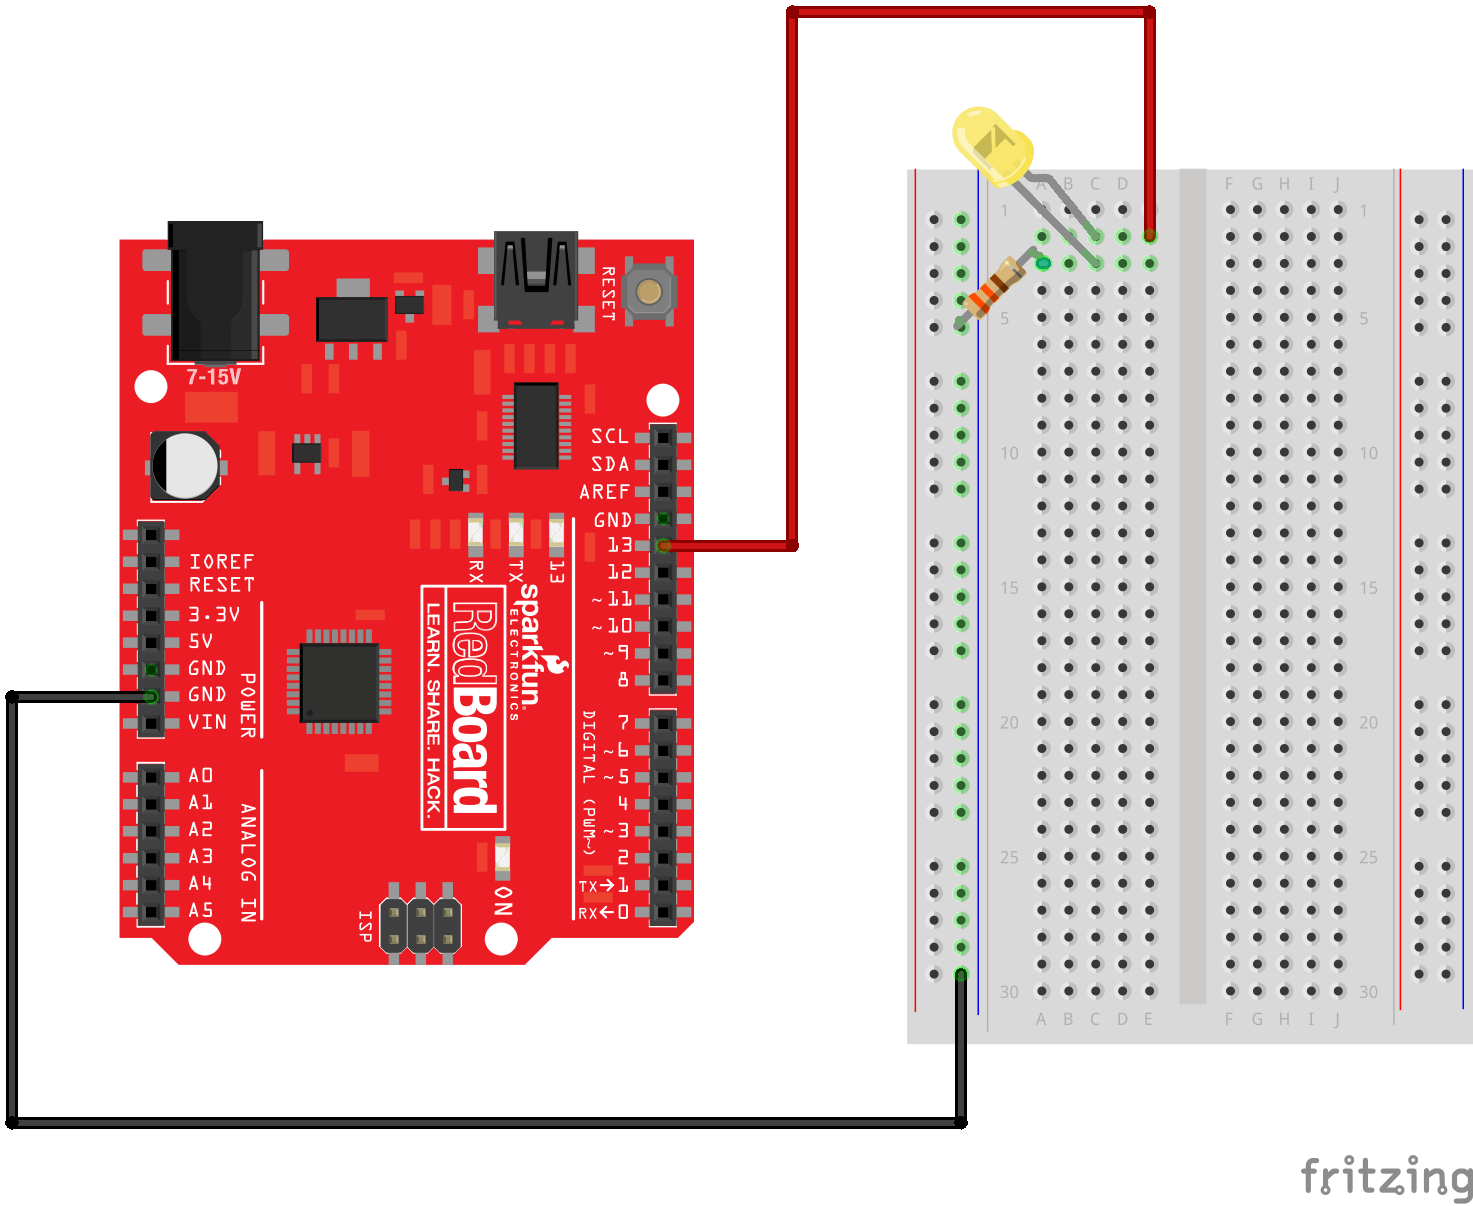
\includegraphics{images/Arduino_LED_fritzing.png}
\caption{Arduino with LED Frizting}
\end{figure}

    \hypertarget{c-upload-the-arduino-example-sketch-blink.ino-onto-the-arduino.-confirm-your-arduino-and-led-blinks.}{%
\paragraph{\texorpdfstring{(c) Upload the Arduino example sketch
\textbf{\emph{Blink.ino}} onto the Arduino. Confirm your Arduino and LED
blinks.}{(c) Upload the Arduino example sketch Blink.ino onto the Arduino. Confirm your Arduino and LED blinks.}}\label{c-upload-the-arduino-example-sketch-blink.ino-onto-the-arduino.-confirm-your-arduino-and-led-blinks.}}

Open the Arduino IDE folder and double click \textbf{Arduino.exe} to
open the Arduino IDE program. In the Arduino IDE, open the
\textbf{\emph{Blink.ino}} sketch by going to: {[}File{]}
--\textgreater{} {[}Examples{]} --\textgreater{} {[}Basics{]}
--\textgreater{} {[}01.Blink{]}.

\begin{figure}[h!]
\centering
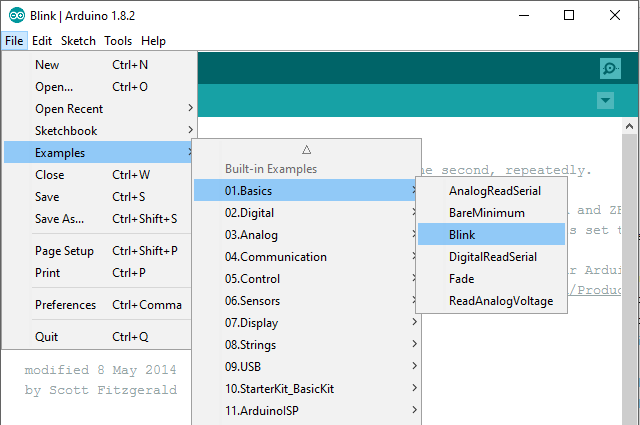
\includegraphics{images/blink_in_examples_menu.png}
\caption{blink.ino in arduino ide}
\end{figure}

Connect the Arduino to the computer using the red USB cable. Note that
USB ports in monitors sometimes do not work correctly with Arduinos. Use
a USB port which is part of the computer. In the Arduino IDE Window that
contains the \textbf{\emph{Blink.ino}} sketch, click the check mark to
Verify, then click the arrow to Upload.

\begin{figure}[h!]
\centering
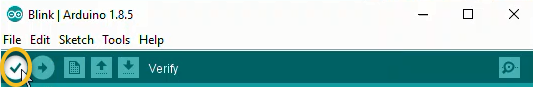
\includegraphics{images/Check_to_Verify.png}
\caption{Check to Verify}
\end{figure}

\begin{figure}[h!]
\centering
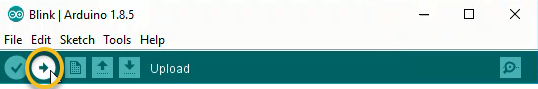
\includegraphics{images/Arrow_to_Upload.png}
\caption{Arrow to Upload}
\end{figure}

Once the upload is complete, the red LED on the Arduino should blink on
and off.

If you don't see the Arduino's LED blinking, you need to do some trouble
shooting:

\begin{itemize}
\tightlist
\item
  Check the COM Port under {[}Tools{]} --\textgreater{} {[}Ports{]}
\item
  Check which type of board is selected under {[}Tools{]}
  --\textgreater{} {[}Board{]}. \textbf{Arduino/Genuino Uno} needs to be
  selected
\item
  Try unplugging and re-plugging in the Arduino's red USB cable. Ensure
  the cable is seated in the computer and Arduino.
\item
  Make sure the Arduino Serial Monitor and Arduino Serial Plotter
  windows are closed
\end{itemize}

    \hypertarget{d-load-the-arduino-example-sketch-physicalpixel.ino}{%
\paragraph{\texorpdfstring{(d) Load the Arduino example sketch
\textbf{\emph{PhysicalPixel.ino}}}{(d) Load the Arduino example sketch PhysicalPixel.ino}}\label{d-load-the-arduino-example-sketch-physicalpixel.ino}}

Open the Arduino \textbf{\emph{PhysicalPixel.ino}} sketch by going to:
{[}File{]} --\textgreater{} {[}Examples{]} --\textgreater{}
{[}04.Communication{]} --\textgreater{} {[}PhysicalPixel{]}.

\begin{figure}[h!]
\centering
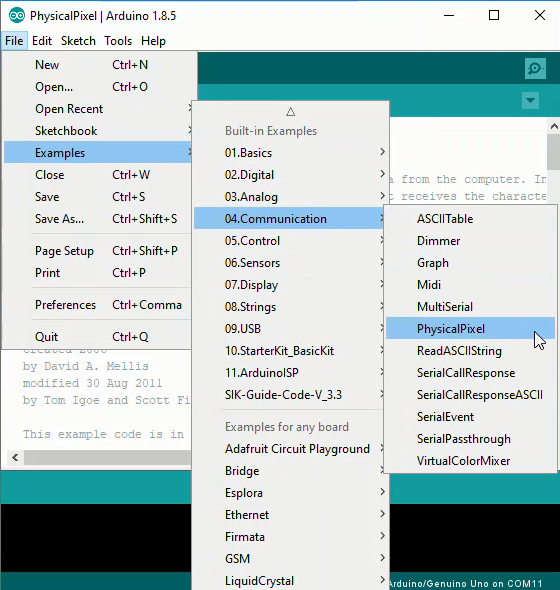
\includegraphics{images/examples_com_physicalpixel.png}
\caption{physicalpixel.ino in the Arduino IDE}
\end{figure}

Once again, In the Arduino IDE Window that contains the PhysicalPixel
sketch, click the check mark to Verify, then click the arrow to Upload.

\begin{figure}[h!]
\centering
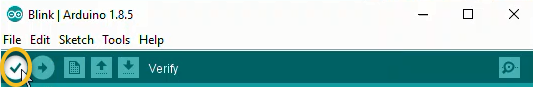
\includegraphics{images/Check_to_Verify.png}
\caption{Check to Verify}
\end{figure}

\begin{figure}[h!]
\centering
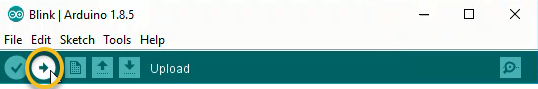
\includegraphics{images/Arrow_to_Upload.png}
\caption{Arrow to Upload}
\end{figure}

    \hypertarget{e-use-the-serial-monitor-to-turn-the-arduino-led-on-and-off}{%
\paragraph{(e) Use the serial monitor to turn the Arduino LED on and
off}\label{e-use-the-serial-monitor-to-turn-the-arduino-led-on-and-off}}

In the Arduino IDE Window that contains the
\textbf{\emph{PhysicalPixel.ino}} sketch, open the Serial Monitor by
going to {[}Tools{]} --\textgreater{} {[}Serial Monitor{]}.

\begin{figure}
\centering
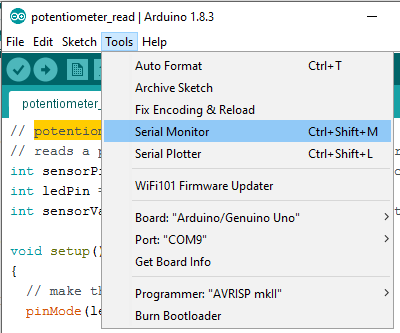
\includegraphics{images/Tools_SerialMonitor.png}
\caption{Tools --\textgreater{} Serial Monitor}
\end{figure}

In the Serial Monitor type: \texttt{H} and click {[}Send{]} (or press
ENTER). Then type: \texttt{L} and click {[}Send{]} (or press ENTER). You
should see the Arduino LED switch on and off. If the LED does not turn
on and off, make sure that the Port is set correctly in {[}Tools{]}
--\textgreater{} {[}Port{]} and make sure that the Serial Monitor is set
to 9600 baud.

\begin{figure}[h!]
\centering
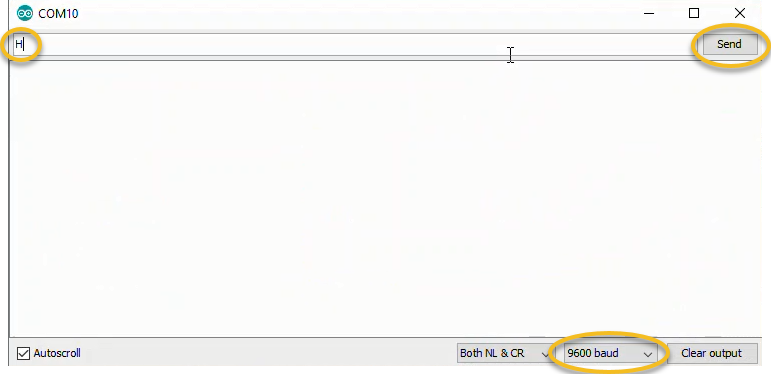
\includegraphics{images/serial_monitor_H.png}
\caption{Send H using the Arduino Serial Monitor}
\end{figure}

If the Arduino is working correctly and the LED can be turned on and off
by typing \texttt{H} and \texttt{L} in the Serial Monitor, close the
Serial Monitor. If the Serial Monitor is left open, Python will not be
able to talk to the Arduino.

    \hypertarget{f-use-the-python-repl-to-turn-the-arduino-led-on-and-off}{%
\paragraph{(f) Use the Python REPL to turn the Arduino LED on and
off}\label{f-use-the-python-repl-to-turn-the-arduino-led-on-and-off}}

Next you are going to use Python to turn the Arduino LED on and off. You
will accomplish this with a Python package called \textbf{PySerial}.
\textbf{PySerial}
(\href{https://pythonhosted.org/pyserial/}{pythonhosted.org/pyserial})
is a Python package used for serial communication. Before you can use
\textbf{PySerial} with Python, the \textbf{PySerial} package needs to be
installed.

The \textbf{PySerial} package can be installed at the \textbf{Anaconda
Prompt}. Go to the Windows Start Menu and search for \textbf{Anaconda
Prompt}. Open an \textbf{Anaconda Prompt} window. At the prompt, type
the following command and hit {[}Enter{]}.

\begin{verbatim}
conda install pyserial
\end{verbatim}

Then type \texttt{y} for yes when prompted.

\begin{figure}[h!]
\centering
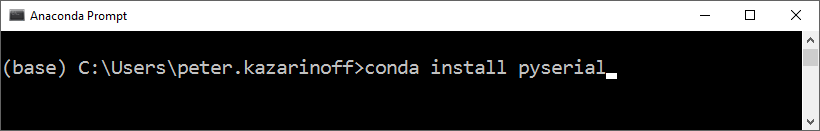
\includegraphics{images/anaconda_prompt_install_pyserial.png}
\caption{Anaconda Prompt showing the command to install PySerial}
\end{figure}

At the Anaconda Prompt, type \texttt{python} to enter the Python REPL
(the Python Prompt).

\begin{figure}[h!]
\centering
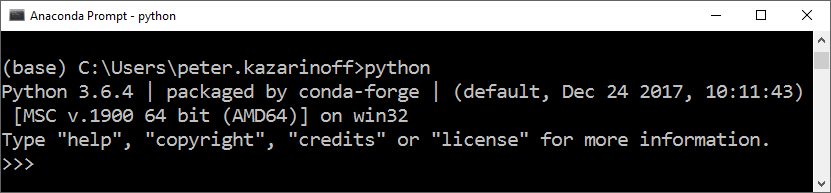
\includegraphics{images/anaconda_prompt_python_REPL.png}
\caption{The Python REPL shown in the Anaconda Prompt}
\end{figure}

At the Python REPL, type the following commands. If the the command is
preceded by a REPL prompt
\texttt{\textgreater{}\textgreater{}\textgreater{}} type the command
into the REPL. If the command does not start with a REPL prompt, this
line represents expected output.

\begin{verbatim}
>>> import serial
>>> import time

>>> ser = serial.Serial('COM4', 9600)  # open serial port
>>> time.sleep(2)                      # wait 2 seconds for connection
>>> ser.name
'COM4'

>>> ser.write(b'H')
# LED turns on

>>> ser.write(b'L')
# LED turns off

>>> ser.write(b'H')
# LED turns on

>>> ser.write(b'L')
# LED turns off

>>> ser.close()
>>> exit()
\end{verbatim}

If you have trouble, check the following:
\begin{itemize}
    \item Make sure the Arduino Serial
Monitor is closed. If the Serial Monitor is left open, Python will not
be able to talk to the Arduino. 
\item Make sure the
\texttt{\textquotesingle{}COM\textquotesingle{}} Port is set correctly.
Open the \textbf{Windows Device Manager} and search under {[}Ports (COM
\& LPT){]} 
\item Make sure the
\texttt{\textgreater{}\textgreater{}\textgreater{}\ ser.close()} command
was called if the serial line was opened before
\item Unplug and re-plug the
red USB cable connected to the Arduino
\end{itemize}

    \hypertarget{f-build-a-python-script-to-turn-the-arduino-led-on-and-off}{%
\paragraph{(f) Build a Python script to turn the Arduino LED on and
off}\label{f-build-a-python-script-to-turn-the-arduino-led-on-and-off}}

If the Arduino is working correctly and the LED can be turned on and off
by typing \texttt{ser.write(b\textquotesingle{}H\textquotesingle{})} and
\texttt{ser.write(b\textquotesingle{}L\textquotesingle{})} at the Python
REPL, make sure to call \texttt{ser.close()} and \texttt{exit()} to
close the serial line and exit out of the Python REPL. If the serial
connection is left open, your Python script will not be able to talk to
the Arduino.

Now construct a Python script called \textbf{\emph{LED.ipynb}} which
turns the Arduino LED on and off, just like you were able to turn the
LED on and off with the Serial Monitor and the Python REPL. To do this,
you have to program Python to send the characters \texttt{L} and
\texttt{H} over the Serial line to the Arduino.

At the start of your Python script, include a comments (\texttt{\#})
section the contains a line with the program title, and separate lines
that contain your name, the lab number and lab name, course quarter and
date. Below the heading section, start your Python code.

The first code section of your script needs to include imports for the
\textbf{PySerial} package and the \textbf{time} module. Include the
lines:

\begin{verbatim}
import serial
import time
\end{verbatim}

The next section of your script needs to set up the serial line for
communication. Note the
\texttt{Port\ =\ \textquotesingle{}COM4\textquotesingle{}} line must be
set according to the port the Arduino is connected to. Insert the code
below:

\begin{verbatim}
ser = serial.Serial('COM4', 9600)  # open serial port
time.sleep(2)

print(ser.name)                    # check which port was really used

# code to run          

ser.close() 
\end{verbatim}

Before you run the open serial port section of code, put in place the
line of code that closes the serial port. If the serial port is not closed,
you will not be able to use the serial port the next time your script
runs. When you have problems connecting to the Arduino with Python,
often it is because the serial line was not closed.

Insert one of the sections of code below between the opening and closing
of the serial port:

\begin{verbatim}
# code to run 

# turns on LED
ser.write(b'H')
time.sleep(1)
\end{verbatim}

or

\begin{verbatim}
# code to run

# turns off LED
ser.write(b'L')
time.sleep(1)
\end{verbatim}

Run the entire Python script to ensure there are no errors and you can open and
close the serial port. A common error is the serial port
\texttt{\textquotesingle{}COM\#\textquotesingle{}} is not set correctly.
Make sure you can the LED turns on and off by running the two sections
of code above.

Next, build a new section of code between the Open serial section and
Close serial section. This section of code sends an
\texttt{\textquotesingle{}H\textquotesingle{}} character over the serial
line waits a second, then sends a
\texttt{\textquotesingle{}L\textquotesingle{}} character over the serial
line and waits another second. The code below is designed to blink the
Arduino LED on and off 10 times.

\begin{verbatim}
# code to run

for t in range(10);
    ser.write(b'H')
    time.sleep(1)
    ser.write(b'L')
    time.sleep(1)
\end{verbatim}

    Run the entire Python script and watch the Arduino LED blink 10 times. A
common problem is the serial port was not closed before the script
starts. Make sure the Arduino Serial Monitor is closed and try running
\texttt{\textgreater{}\textgreater{}\textgreater{}\ ser.close()} at the
Python REPL.

Once Python successfully blinks the Arduino LED, use your Python coding
skills to ask the user for input and turn on or off the Arduino's LED
based on user input. Complete this task with the \texttt{input()}
function running in a \textit{while loop}. Within the while loop, add an \textit{if
statement} that allows the program to break out of the loop (remember the
keyword \texttt{break}) and go to the \texttt{ser.close()} section. Remember, the
serial port must be closed for Python to use the serial line again.

Below is an example of an if/break statement:

\begin{verbatim}
if user_input == 'q':
    break 
\end{verbatim}

When your Python script runs, the user should see functionality like
below:

\begin{verbatim}
>>> Type H to turn on the LED, L to turn off the LED or q to quit: H
[LED TURNS ON]
>>> Type H to turn on the LED, L to turn off the LED or q to quit: L
[LED TURNS OFF]
>>> Type H to turn on the LED, L to turn off the LED or q to quit: q
[PROGRAM TERMINATES]
\end{verbatim}

    \hypertarget{part-2.-measure-sensor-output-with-python-and-an-arduino}{%
\subsubsection{Part 2. Measure sensor output with Python and an
Arduino}\label{part-2.-measure-sensor-output-with-python-and-an-arduino}}

Once you have completed Part 1 of the lab and can turn the Arduino LED
on and OFF using Python continue on to Part 2. In Part 2 of the lab, you
will use Python to read a sensor (a potentiometer dial) connected to the
Arduino and plot the data using Matplotlib.

    \hypertarget{a-wire-a-potentiometer-dial-to-the-arduino}{%
\paragraph{(a) Wire a potentiometer dial to the
Arduino}\label{a-wire-a-potentiometer-dial-to-the-arduino}}

First, you need to connect connect the potentiometer to the Arduino. You
should leave your LED and resistor attached as you will use the LED and
resistor with the potentiometer. \textbf{Unplug the red Arduino USB
cable} and connect the small blue potentiometer dial to your Arduino as
shown below. Also see the SIK GUIDE page 25 and the SparkFun Iventor's
kit online guide:

\begin{quote}
\href{https://learn.sparkfun.com/tutorials/sparkfun-inventors-kit-experiment-guide---v40/circuit-1b-potentiometer}{https://learn.sparkfun.com/tutorials/sparkfun-inventors-kit-experiment-guide---v40/circuit-1b-potentiometer}
\end{quote}

\begin{figure}[h!]
\centering
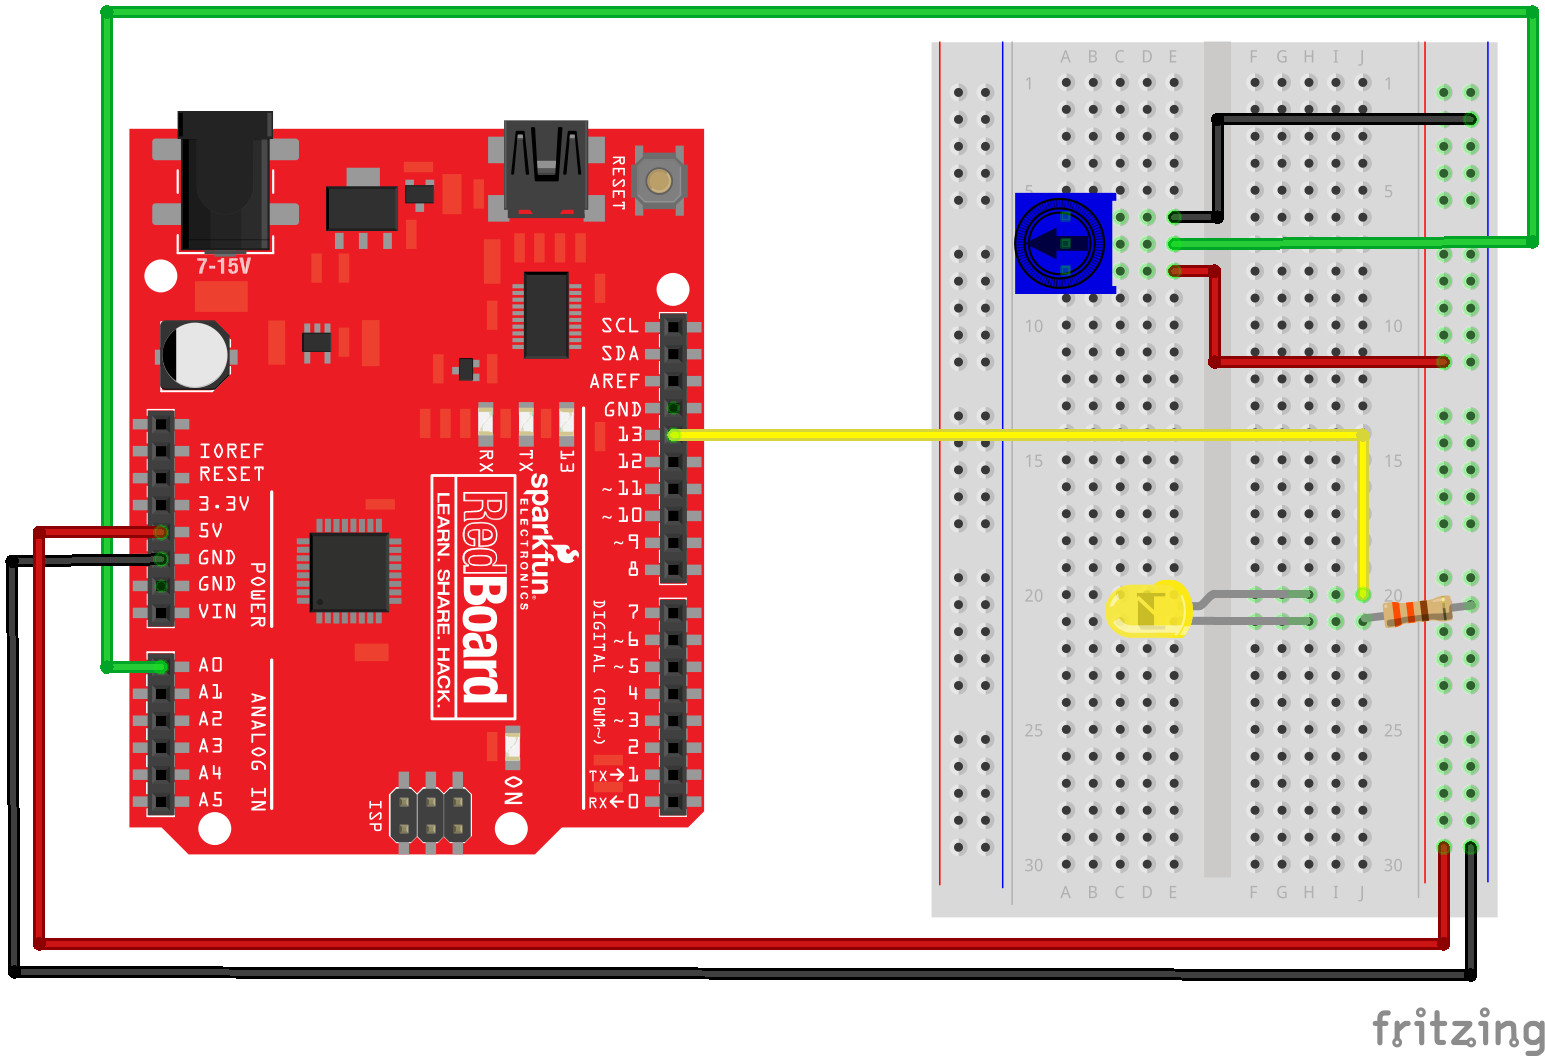
\includegraphics{images/redboard_pot_led_fritzing.png}
\caption{Arduino Potentiometer Fritzing Schematic}
\end{figure}

\newpage

    \hypertarget{b-copy-and-load-the-potentiometer.ino-sketch-onto-the-arduino}{%
\paragraph{\texorpdfstring{(b) Copy and load the
\textbf{\emph{potentiometer.ino}} sketch onto the
Arduino}{(b) Copy and load the potentiometer.ino sketch onto the Arduino}}\label{b-copy-and-load-the-potentiometer.ino-sketch-onto-the-arduino}}

Open a new sketch in the Arduino IDE by going to {[}File{]}
--\textgreater{} {[}New{]}. Copy the code below into the new sketch and
save the sketch as \textbf{\emph{potentiometer.ino}}

\begin{verbatim}
// potentiometer_read.ino
// reads a potentiometer and sends value over serial

int sensorPin = A0; // The potentiometer is connected to analog pin 0
int ledPin = 13; // The LED is connected to digital pin 13
int sensorValue; // an integer variable to store the potentiometer reading

void setup() // this function runs once when the sketch starts
{
// make the LED pin (pin 13) an output pin
pinMode(ledPin, OUTPUT);
// initialize serial communication at 9600 baud
Serial.begin(9600);
}

void loop() // this function runs repeatedly after setup() finishes
{
sensorValue = analogRead(sensorPin); // read the voltage at pin A0
Serial.println(sensorValue); // Output voltage value to Serial Monitor
if (sensorValue < 500) { // if sensor output is less than 500,
digitalWrite(ledPin, LOW); } // Turn the LED off
else {                   // if sensor output is greater than 500
digitalWrite(ledPin, HIGH); } // Keep the LED on
delay(100); // Pause 100 milliseconds before next reading
}
\end{verbatim}

\textbf{Plug the red USB cable back into the Arduino and computer.} In
the Arduino IDE window that contains the potentiometer
\textbf{\emph{potentiometer.ino}} sketch, click the check mark to Verify
the click the arrow to Upload.

    \hypertarget{c-twist-the-potentiometer-to-turn-the-led-connected-to-the-arduino-on-and-off}{%
\paragraph{(c) Twist the potentiometer to turn the LED connected to the
Arduino on and
off}\label{c-twist-the-potentiometer-to-turn-the-led-connected-to-the-arduino-on-and-off}}

After the potentiometer \textbf{\emph{potentiometer.ino}} sketch is
uploaded to the Arduino, twist the small blue potentiometer dial back
and forth and watch the LED turn on and off (the dial can be stiff). The
on/off point should be about half way through the little blue
potentiometer's rotation. If the LED does not turn on and off, double
check your wiring and try uploading the
\textbf{\emph{potentiometer.ino}} sketch again. Ensure the Serial
Monitor is closed and that Python closed the Serial Port before you
upload the sketch.

    \hypertarget{d-use-the-arduino-serial-monitor-and-serial-plotter-to-see-the-potentiometer-reading}{%
\paragraph{(d) Use the Arduino Serial Monitor and Serial Plotter to see
the potentiometer
reading}\label{d-use-the-arduino-serial-monitor-and-serial-plotter-to-see-the-potentiometer-reading}}

Open the Arduino Serial Monitor in the Arduino IDE by going to
{[}Tools{]} --\textgreater{} {[}Serial Monitor{]}.

\begin{figure}[h!]
\centering
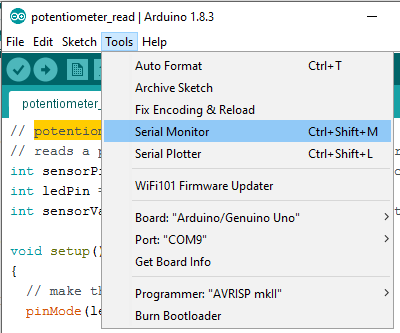
\includegraphics{images/Tools_SerialMonitor.png}
\caption{Arduino Tools --\textgreater{} Serial Monitor}
\end{figure}

You should see numbers scrolling down the Serial Monitor if the
potentiometer \textbf{\emph{potentiometer.ino}} sketch is working
properly. Twist the little blue potentiometer and watch the numbers
scrolling down the Serial Monitor change.

\begin{figure}[h!]
\centering
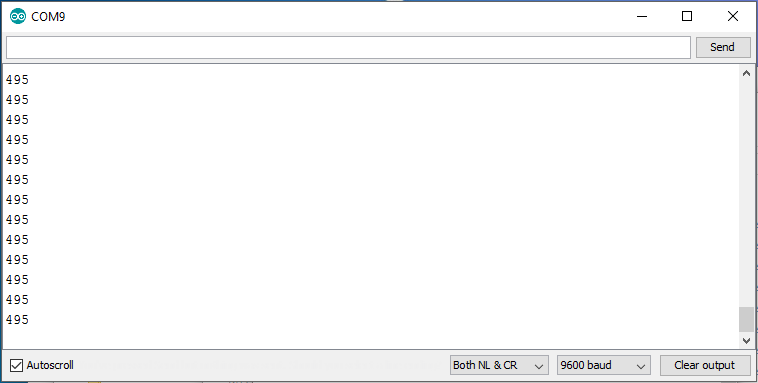
\includegraphics{images/serial_monitor_output.png}
\caption{Arduino Serial Monitor}
\end{figure}

Close the Arduino Serial Monitor and open the Arduino Serial
Plotter by going to {[}Tools{]} --\textgreater{} {[}Serial Plotter{]}.

\begin{figure}[h!]
\centering
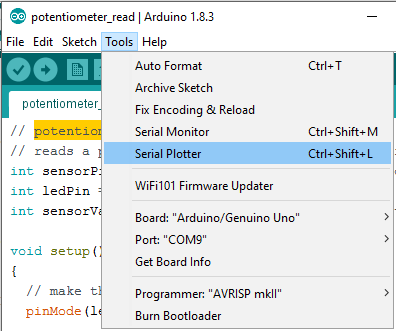
\includegraphics{images/Tools_SerialPlotter.png}
\caption{Arduino Tools --\textgreater{} Serial Plotter}
\end{figure}

You should see a plot with a moving line. Twist the little blue
potentiometer and observe the line on the plot move up and down.

If the Serial Plotter works, close the Serial Plotter Window. If Serial
Plotter isn't working, make sure the
\texttt{\textquotesingle{}COM\textquotesingle{}} port is set correctly
in the Arduino IDE, and ensure the serial port was closed by Python. The
Arduino Serial Monitor and Serial Plotter can not be open at the same
time, and both need to be closed before Python can communicate with the
Arduino.

\begin{figure}[h!]
\centering
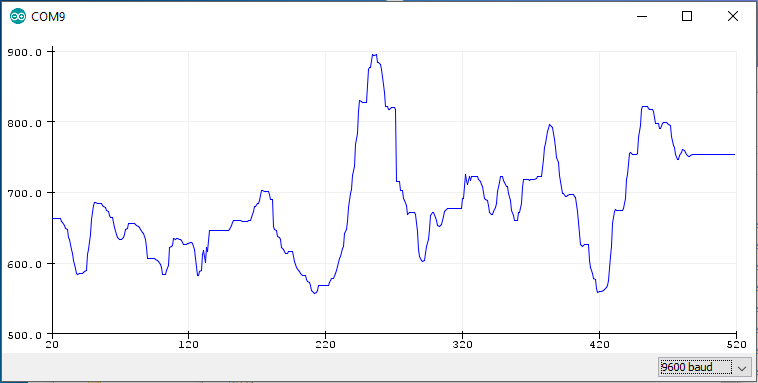
\includegraphics{images/serial_plotter_output.png}
\caption{Arduino Serial Plotter}
\end{figure}

    \hypertarget{e-use-the-python-repl-to-read-the-potentiometer-data}{%
\paragraph{(e) Use the Python REPL to read the potentiometer
data}\label{e-use-the-python-repl-to-read-the-potentiometer-data}}

Open the \textbf{Anaconda Prompt}, type \texttt{python} to enter the
Python REPL.

\begin{figure}[h!]
\centering
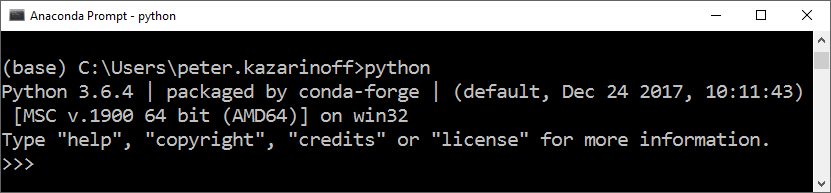
\includegraphics{images/anaconda_prompt_python_REPL.png}
\caption{The Python REPL shown in the Anaconda Prompt}
\end{figure}

At the Python REPL, type the following commands. If the command is
preceded by a REPL prompt
\texttt{\textgreater{}\textgreater{}\textgreater{}} type the command
into the REPL. If the line does not start with a REPL prompt, this line
represents expected output.

\begin{verbatim}
# serial read using the Python REPL

>>> import serial
>>> import time
>>> ser = serial.Serial('COM4', 9600)
>>> time.sleep(2)
>>> b = ser.readline()
>>> b
b'409\r\n'
>>> type(b)
<class 'bytes'>
>>> str_rn = b.decode()
>>> str_rn
'409\r\n'
>>> str = str_rn.rstrip()
>>> str
'409'
>>> type(str)
<class 'str'>
>>> f = float(str)
>>> f
409.0
>>> type(f)
<class 'float'>
>>> ser.close()
>>> exit()
\end{verbatim}

Note how the data read over the serial line was converted into different
data types. The data came in as
\texttt{\textless{}class\ \textquotesingle{}bytes\textquotesingle{}\textgreater{}}.
The data was then converted to a Python string
\texttt{\textless{}class\ \textquotesingle{}str\textquotesingle{}\textgreater{}}.
Then the \texttt{\textbackslash{}r\textbackslash{}n} characters were
removed, and finally the string was converted to a float
\texttt{\textless{}class\ \textquotesingle{}float\textquotesingle{}\textgreater{}}.

    \hypertarget{f-build-a-python-script-and-to-record-the-potentiometer-level-and-draw-a-plot}{%
\paragraph{(f) Build a Python script and to record the potentiometer
level and draw a
plot}\label{f-build-a-python-script-and-to-record-the-potentiometer-level-and-draw-a-plot}}

After you can successfully:

\begin{itemize}
\tightlist
\item
  turn the Arduino LED on and off by twisting the little blue
  potentiometer
\item
  see the values changing in the Arduino Serial Monitor when the little
  blue potentiometer is turned
\item
  see the plot line moving up and down in the Arduino Serial Plotter when the
  little blue potentiometer is turned
\item
  read a data from the serial line and convert the data to a float
\end{itemize}

The next step is to build a Python script that reads the
potentiometer data and builds a plot (like the plot you see in the
Arduino Serial Plotter).

To read the potentiometer value with Python, create a new script called
\textbf{potentiometer.ipynb}. At the start of the Python script include
the standard header with comment lines \texttt{\#} which includes a line
for a title, and lines for your name, the lab number and name,
course/quarter and date.

The first lines of code in the script need to import the
\textbf{PySerial} package and and the \textbf{time} module:

\begin{verbatim}
import serial
import time
\end{verbatim}

The next section of the Python script needs to set up the serial line
for communication and read the sensor value from the potentiometer. Note
the Port (\texttt{\textquotesingle{}COM4\textquotesingle{}}) must be set
according to the port the Arduino is connected to.

\begin{verbatim}
# set up the serial line
ser = serial.Serial('COM4', 9600)
time.sleep(2)
print(ser.name)

# Read and record the data
data =[]                           # initialize and empty list to store the data
for i in range(50):
    b = ser.readline()             # read a byte string line from the Arduino's serial output
    string_n = b.decode()          # decode byte string into regular Python string
    string = string_n.rstrip()     # remove \n and \r from the string
    flt = float(string)            # convert the string to a float
    print(flt)
    data.append(flt)               # add the float to the end of the data list
    time.sleep(0.1)                # wait (sleep) 0.2 seconds before the next reading

ser.close()

# Plot the data
\end{verbatim}

Run the script and twist the potentiometer. You should see the
potentiometer values running by in the Python REPL command window.

Finally, fill in the remaining two sections in the script. Include a
section that asks a user for how long to collect data. Limit the user to
a maximum of 60 seconds. Then include a section that plots the
potentiometer reading vs.~time using Matplotlib. Note that the data is
recorded every 10th of a second.

When the Python script runs, it should function in the following way:

\begin{verbatim}
Enter the number of seconds to record data (0 - 60) : 10
\end{verbatim}

\begin{figure}[h!]
\centering
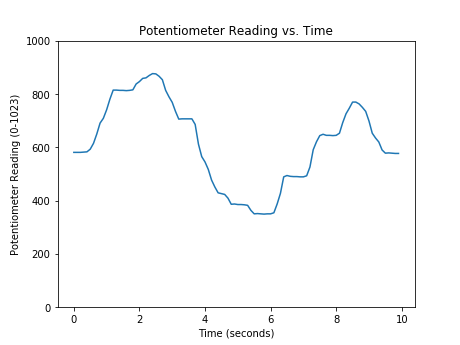
\includegraphics{images/potentiometer_reading.png}
\caption{Example Matplotlib plot of potentiometer data}
\end{figure}

    \hypertarget{going-further}{%
\subsubsection{Going further}\label{going-further}}

If you have time, there is some additional functionality you can add to
your Python script:

\begin{itemize}
\item
  Display the high and low potentiometer readings
\item
  Connect a photocell to the Arduino and plot photocell readings with
  Python
\item
  Build a dynamic plot using an animated line that moves as the
  potentiometer value changes
\end{itemize}

    \hypertarget{deliverables}{%
\subsection{Deliverables}\label{deliverables}}

Make sure your group's Python and Arduino code are well commented and
sectioned. Ensure the variable names are descriptive and there is enough
documentation for another group of students to reuse the code without
much trouble. Each student's submission for the lab should be a pair of the
following files (you do not need to submit all the
\textbf{\emph{.ipynb}} and \textbf{\emph{.ino}} files used in the lab,
just submit the files you were primarily responsible for).

Each student needs to upload one Python file (one .ipynb-file) and one
Arduino file (one .ino-file):

\textbf{\emph{LED.ipynb}} and \textbf{\emph{PhysicalPixel.ino}}

or

\textbf{\emph{potentiometer.ipynb}} and
\textbf{\emph{potentiometer.ino}}

Upload your files to the D2L Lab 8 Uploads
folder.
    % Add a bibliography block to the postdoc
    
    
    
    \end{document}
